
\chapter{Future Work}
\label{sec:future_work}

This chapter explains what will be done in the remaining time of the project. It talks about some of the long term goals and the activities that will be carried to achieve them.

\section{Schedule}
\label{sec:schedule}

For the next months it is expected to have the script for SDL2 projects finished with support for Windows and MacOS. The known issues described on Section \ref{sec:issues} have to be fixed for both SDL 1 and 2. The building scripts have to be tested against all the available games.

Another goal is to allow the user to link their GitHub repository to the website, letting them build the packages for the game automatically with GitHub hooks. The game will then, be available in the website without the need for a manual upload from an administrator.

It's also purpose of this next part of the semester to maintain and evolve the platform while the tasks related to the script are being held. Some selected issues will be resolved to add new features and fix bugs found on the system.

The following activities will be developed in the remaining time of the project. They are summarized in Figure \ref{fig:schedule}.

\begin{enumerate}
\item \textbf{Literature Review}: review what the literature has on packaging, CMake, game development.
\item \textbf{Add Lua support}: some of the games, especially the ones built with SDL2, have lua as a dependency library. This lib is not being being compiled in the current version of the building scripts.
\item \textbf{Add other Linux distros support}: allow other users to install the games using their package manager. Generate at least \textit{.rpm} packages in addition to the \textit{.deb} already generated.
\item \textbf{Add Darcy's games}: look for games developed at Darcy Ribeiro campus and run the building scripts on them.
\item \textbf{Add MacOS support}: create install packages for Mac (Apple Systems).
\item \textbf{Add Windows support}: make an installer (\textit{.exe}) to run on Windows 10 (maybe with some backwards compatibility if possible).
\item \textbf{Integrate to platform}: run the scripts though a request on the website
\item \textbf{Avoid duplication on save}: according to the GitHub repository of the team, models are being saved with duplicated data.
\item \textbf{Create games statistics}: create endpoints to send game statistics, like views and download amounts.
\item \textbf{Submit issues to the GitHub repository}: allow users to submit issues through the platform to the GitHub repository of the game.
\item \textbf{Integrate to GitHub}: make the system receive GitHub signals.
\item \textbf{Allow user to build a game from a branch}: et the user upload a game based on a chosen branch. This will in fact run the script to build the game, but without the need of a an administrator.
\item \textbf{Read game info from game branch}: developers, description and even some images are usually available in the game repository. This task is to read that information to avoid the need of manual input of the administrator.
\item \textbf{Code refactoring}: integrate scripts (SDL 1 and 2), make them more generic and efficient.
\item \textbf{Final adjustments}: make minor improvements and fixes.
\item \textbf{Write Report}: report progress and results.
\end{enumerate}

\begin{figure}[h!]
\centering
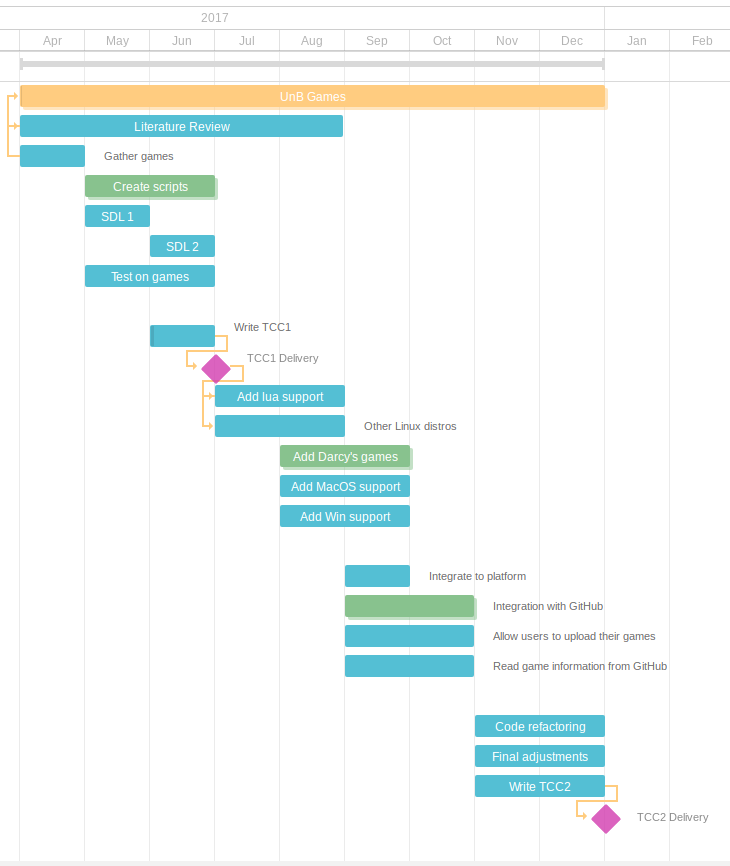
\includegraphics[width=\textwidth,height=\textheight,keepaspectratio]{gantt_chart}
\caption{Project Schedule}
\label{fig:schedule}
\end{figure}
